\chapter{Methodology}

\section{Use case diagram}

\begin{figure}[htb]
\centering
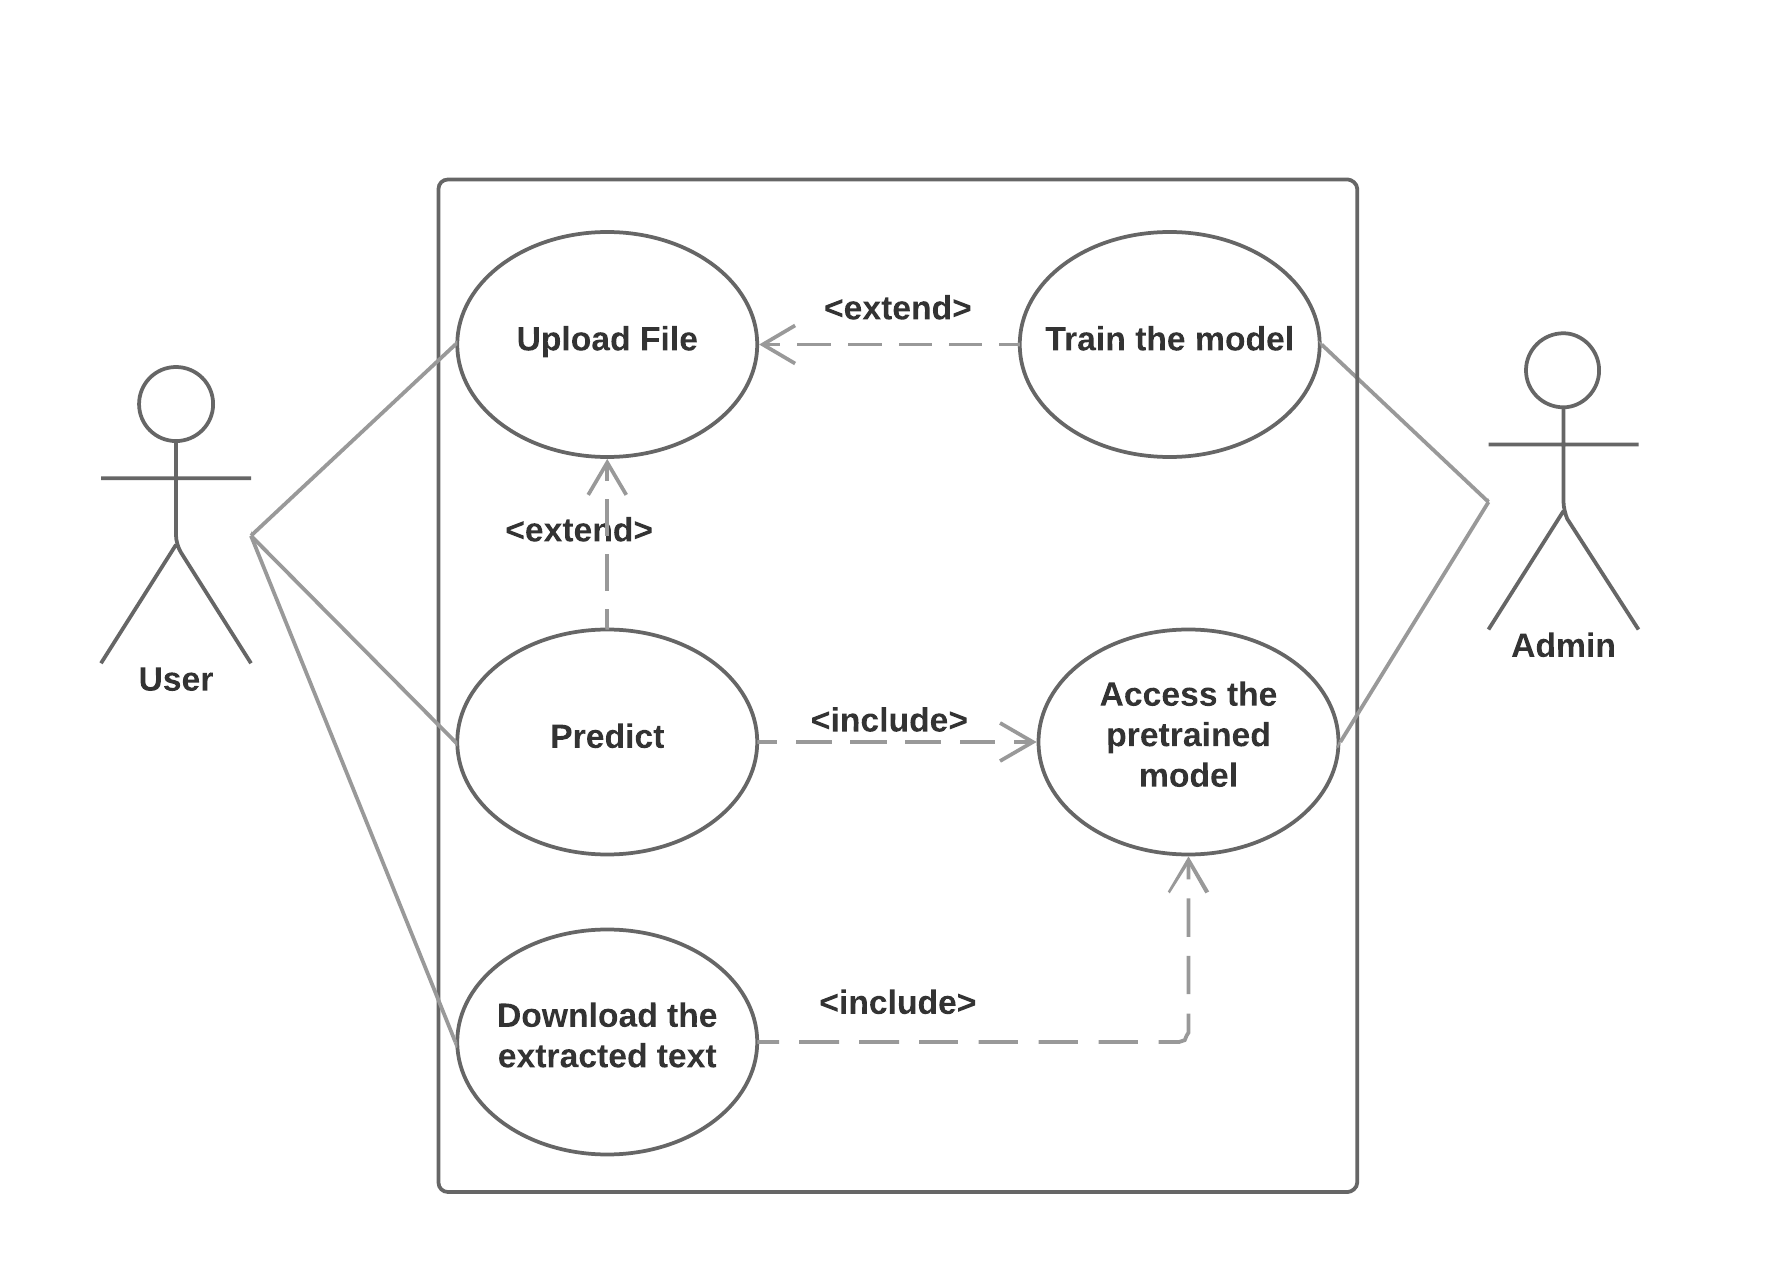
\includegraphics[scale=1]{UseCase}
\caption{Use Case diagram}
\end{figure}

The purpose of a use case diagram here is to demonstrate the different ways that a user might interact with a system. The main actors in our systems are the actual users who use it and the administrator responsible for updating or training the model used in the system. The user uses the system in order to predict the text present in the image by uploading the image and gets the output from the prediction model as indicated in the relationship above.

Also, after the user chooses to predict the text in the image, the pre-trained model is automatically accessed to produce the required output as shown by the relationship between the two use cases.

\section{Level 0 Data Flow Diagram}

\begin{figure}[htb]
\centering
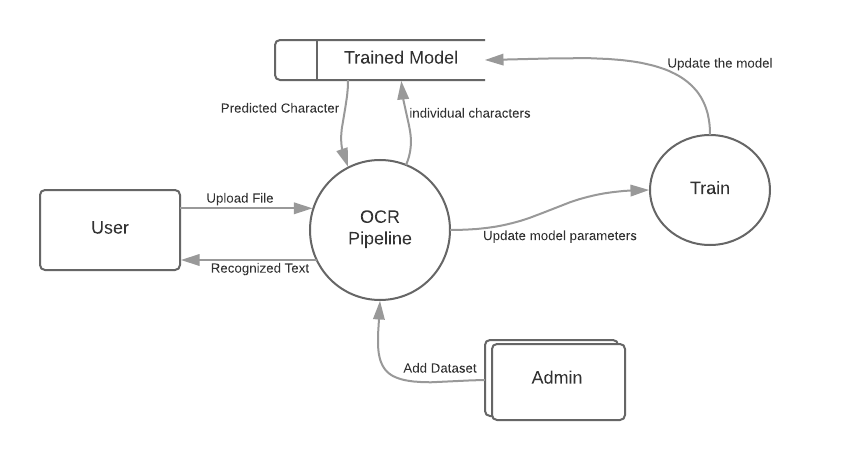
\includegraphics[scale=1]{level0}
\caption{Level 0 Data Flow Diagram}
\end{figure}

DFD Level 0, also called Context Diagram, shows a basic overview of the whole system. The above diagram provides an at-a-glance view, showing the system as a single high-level process, with its relationship to external entities. The circles in the diagram represent a process, the rectangular boxes represent entities and the arrows indicate the data flow direction.

In our system, the external entities are the user and the admin. The OCR pipeline and the trained model are internal to the system. The user directly interacts with the pipeline giving image file as an input and gets the desired output in the form of text from the pipeline. Similarly the admin also interacts with the pipeline with the help of dataset that is used for training as well as testing purposes. Further, the pipeline interacts with the trained prediction model to generate the approximate match of the input character. It can also train the model using the dataset provided by the administrator.

\section{Level 1 Data Flow Diagram}

\begin{figure}[htb]
\centering
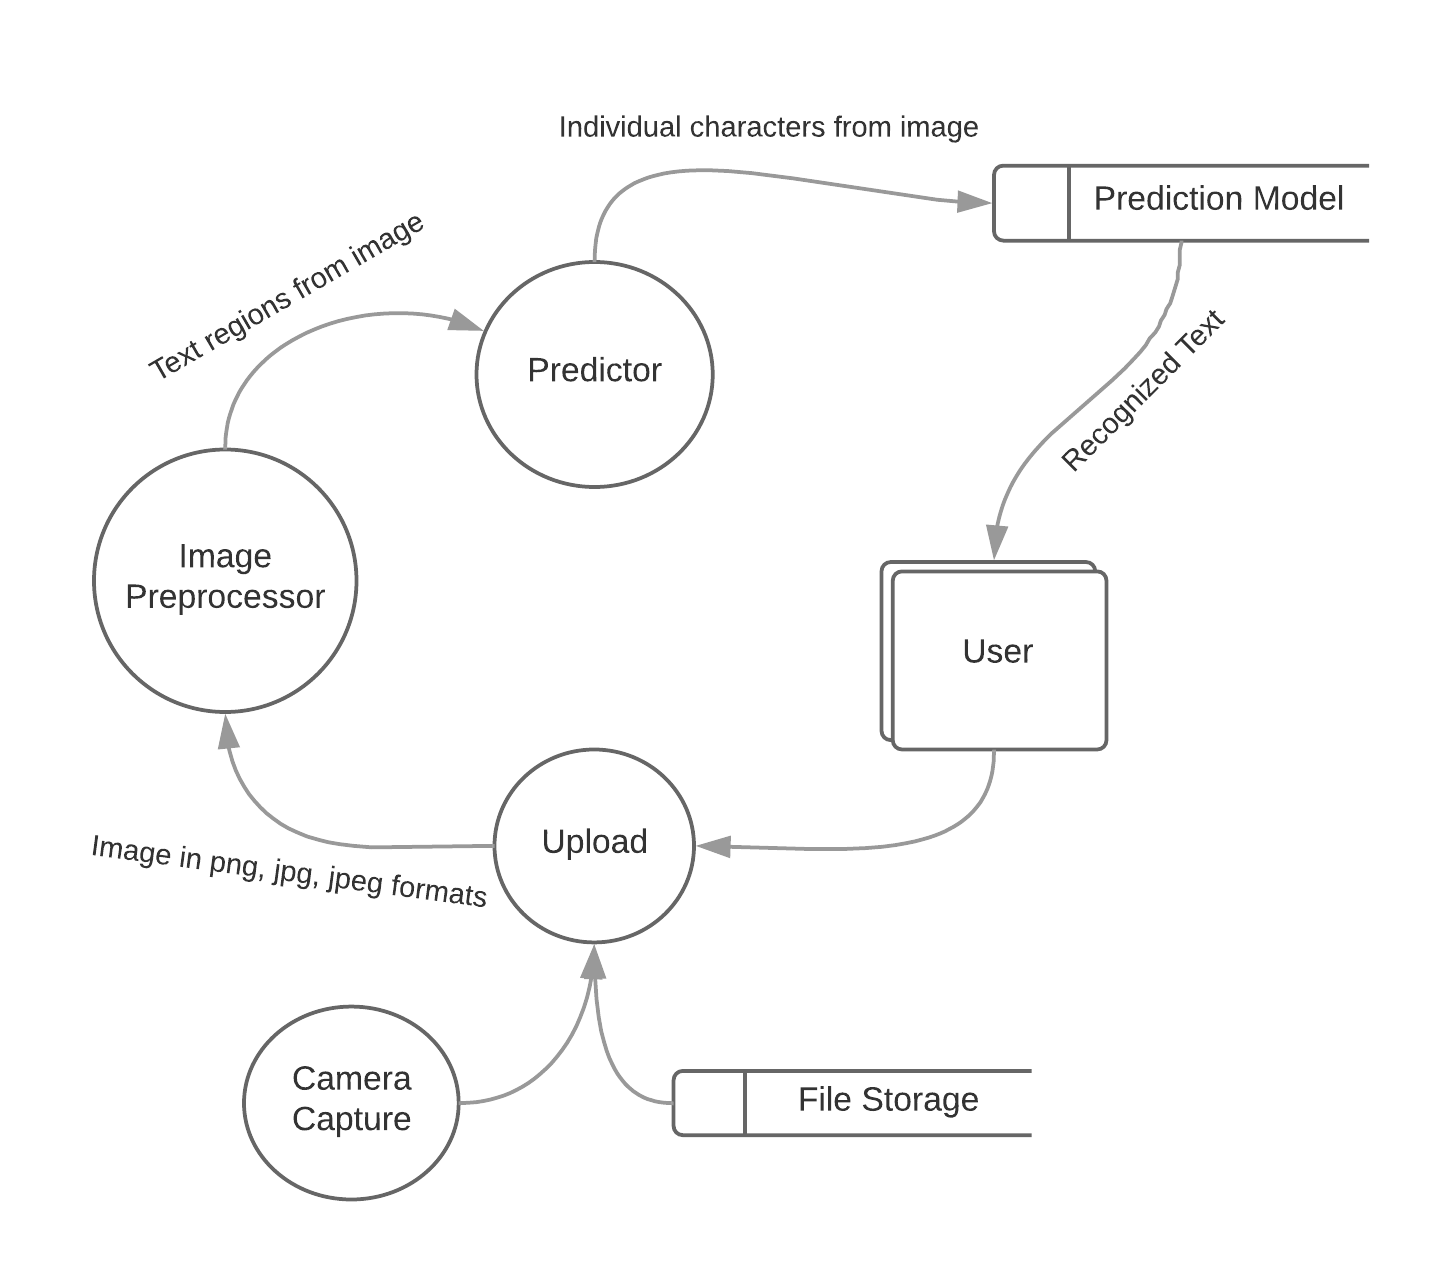
\includegraphics[scale=1]{level1}
\caption{Level 1 Data Flow Diagram}
\end{figure}


DFD Level 1 provides a more detailed breakout of pieces of the Context Level Diagram. The above level 1 DFD diagram of our system shows the OCR pipeline in more detail.

It includes an input mechanism through an external device like camera or through a file storage unit. The OCR pipeline consists of an image processor unit which applies various image processing algorithms to the image to identify text regions in the image. The next processes consists of predicting the text regions with the individual characters separated from the image and updating the user of the identified texts present in the image. 



\section{Level 2 Data Flow Diagram}

DFD Level 2 goes one step deeper into parts of Level 1. 

\begin{figure}[htb]
\centering
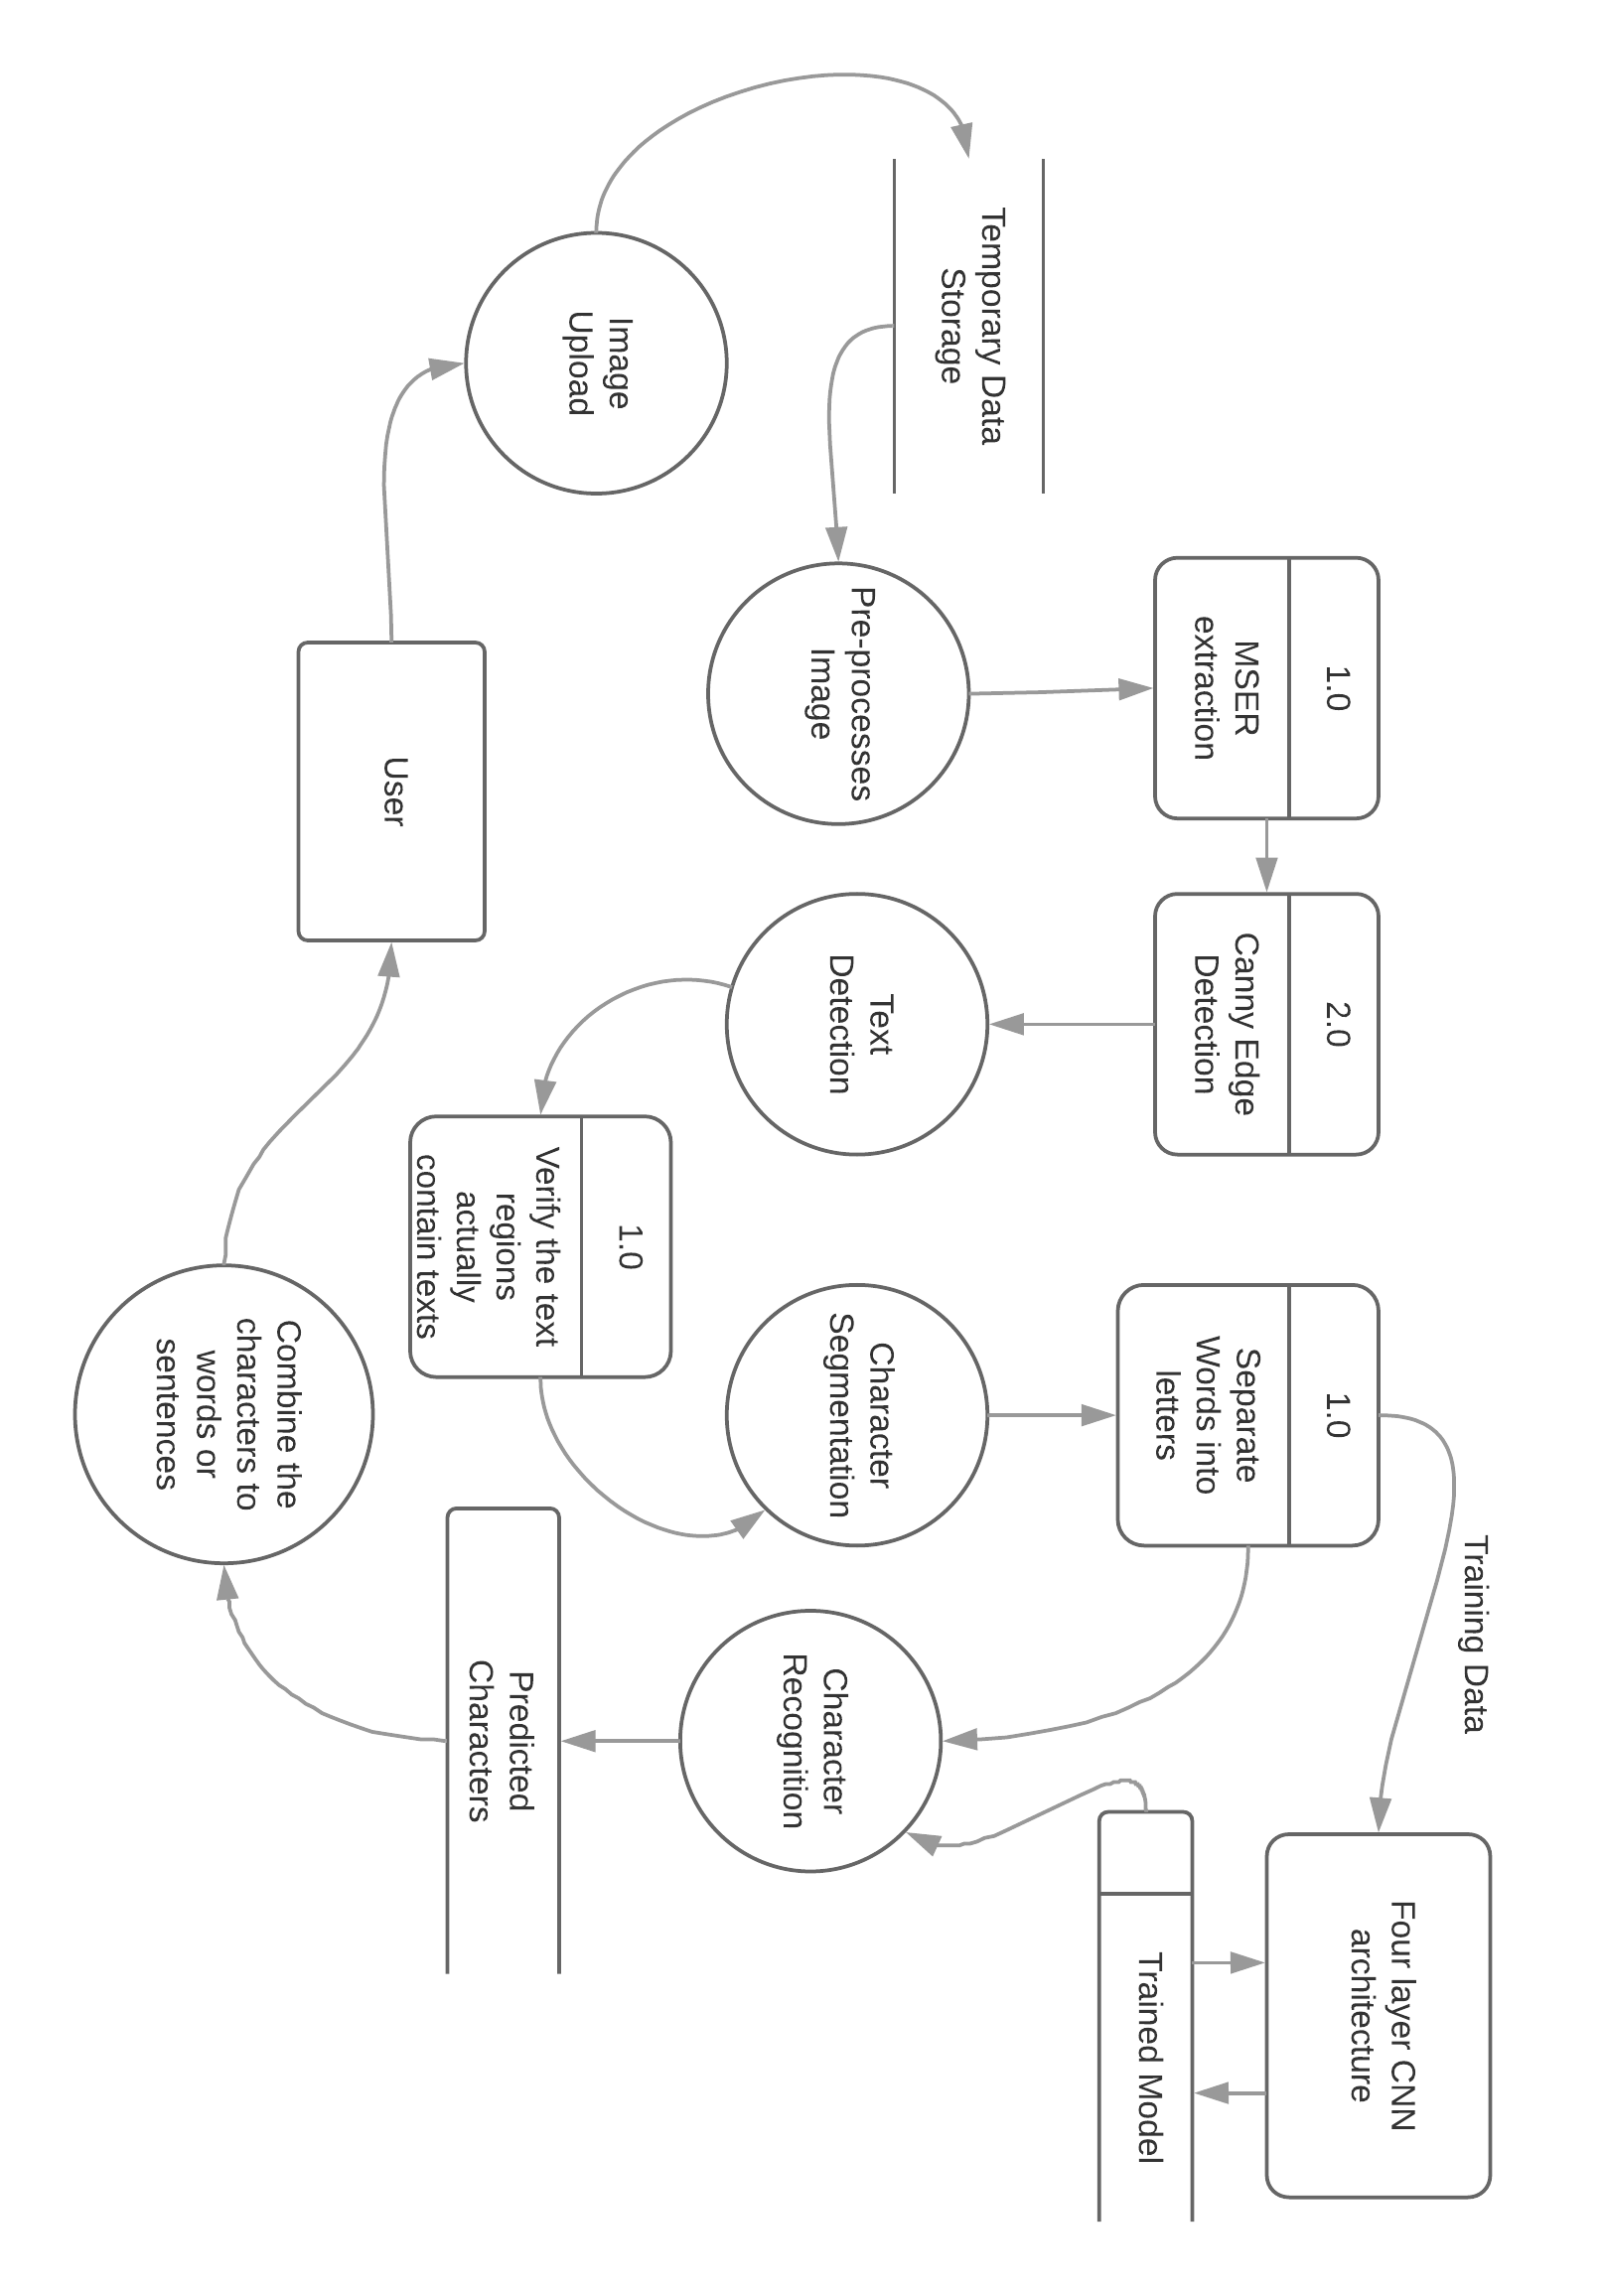
\includegraphics[scale=1]{level2}
\caption{Level 2 Data Flow Diagram}
\end{figure}

Thus the OCR pipeline from Level 1 is further divided into its constituent’s parts. The user interacts with the system using a web interface to upload the image file as well as get the output of the system. The image is then pre-processed using binarization, extraction using a combination of MSER and Canny Edge detection. After the text regions are obtained the regions gets segmented into characters and fed into the recognition engine. The recognition engine uses a pre-trained model trained by a four layer CNN architecture to predict the approximate output of the character or text. The predicted characters are combined to form words or sentences that is displayed to the user.

\section{Entity Relationship Diagram}

\begin{figure}[htb]
\centering
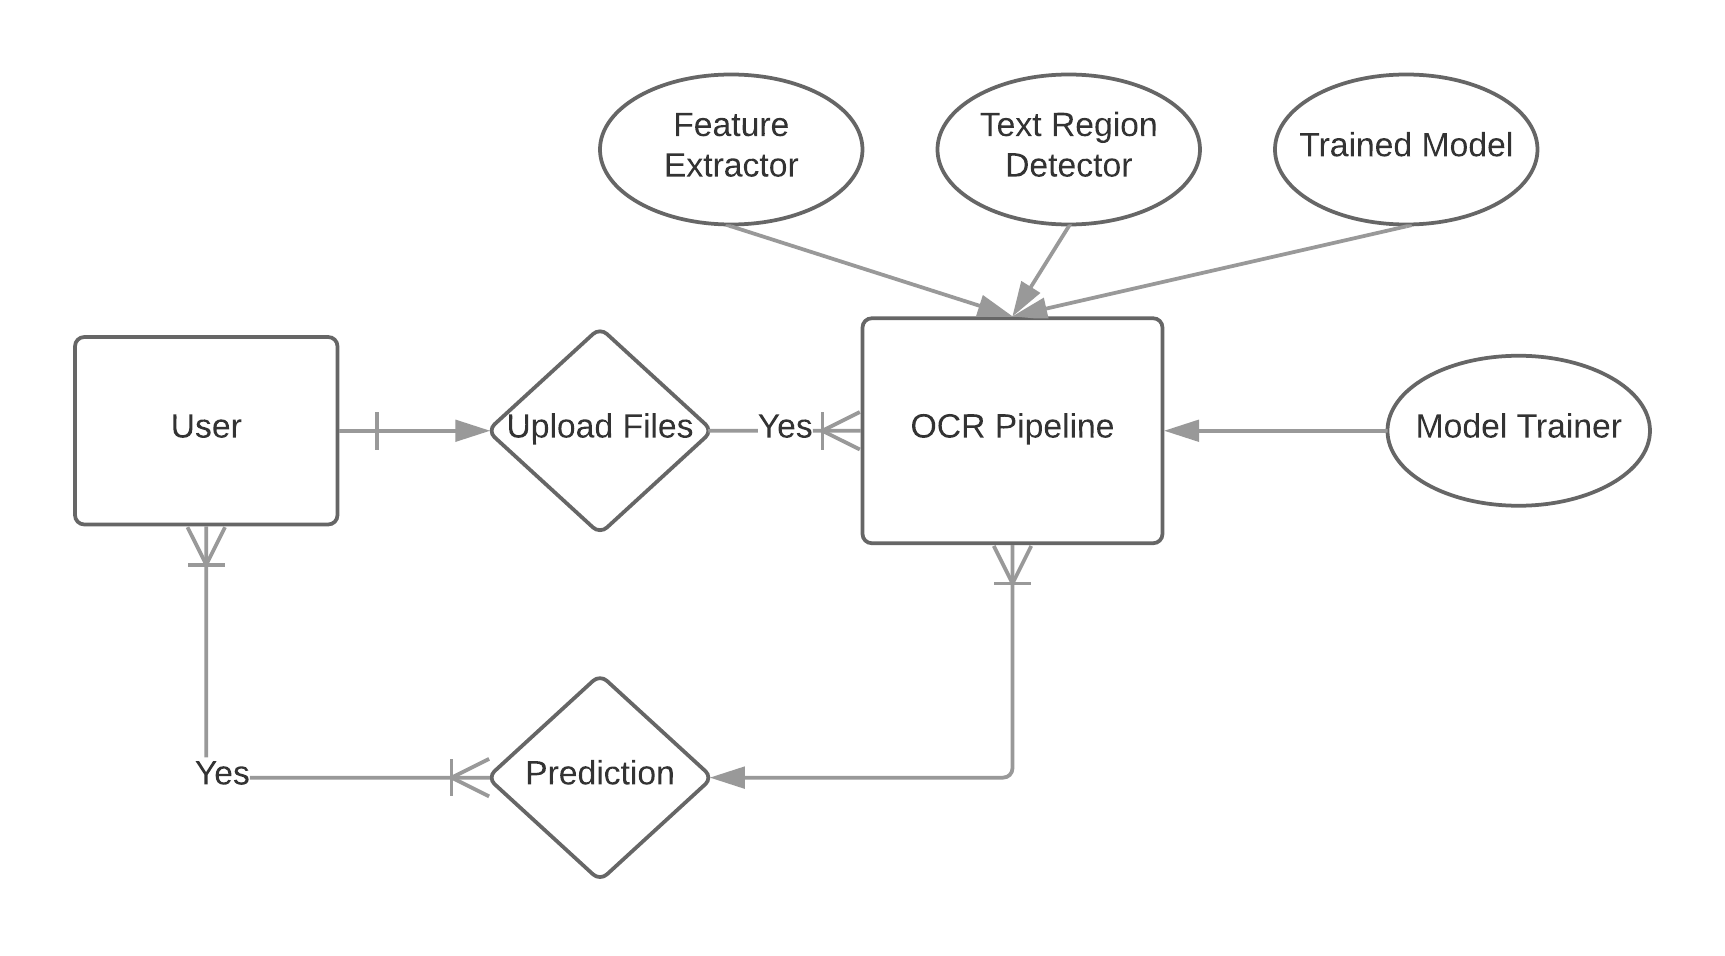
\includegraphics[scale=0.7]{ERD}
\caption{Entity Relationship Diagram}
\end{figure}


An Entity Relationship (ER) diagram shows how entities like people, objects, or concepts relate to each other within a system. In an ER diagram, the rectangular boxes represent the objects, or entities, diamonds represent the relationship between the entities, and an oval represents an attribute of an entity.

In the proposed system we have two major entities the user and the OCR pipeline. A user can upload one or many files at a time to the system. The pipeline has various components that analyses the given image and prints the gives the output of the images to on or many users. 

\section{Activity Diagram}

\begin{figure}[htb]
\centering
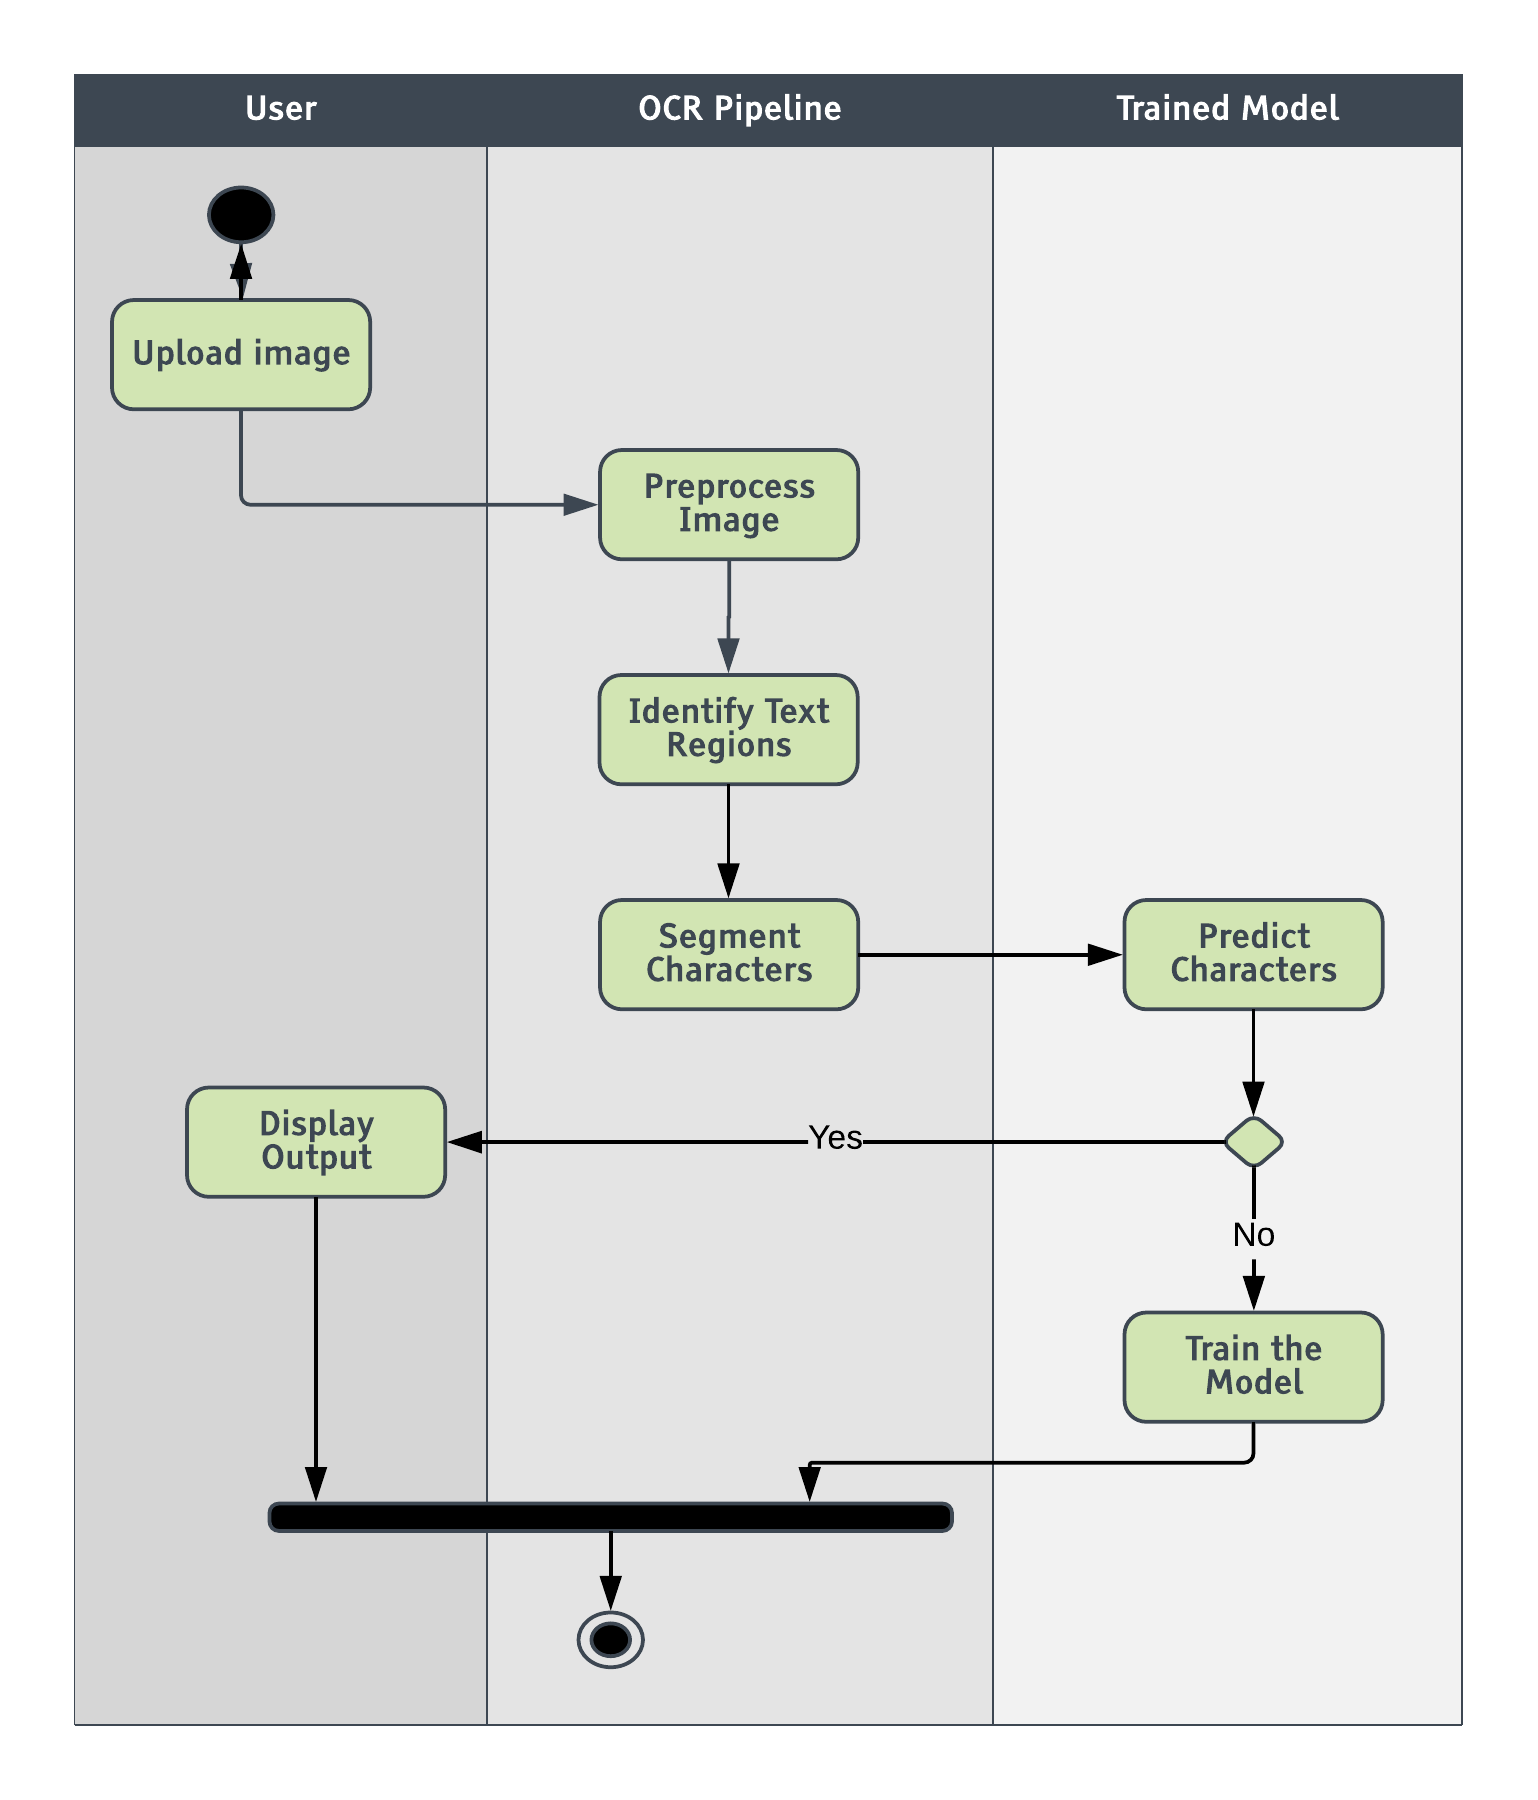
\includegraphics[scale=0.7]{Activity}
\caption{Activity Diagram}
\end{figure}

An activity diagram is essentially a flowchart that shows activities performed by a system. 
The major activities in our system is outlined in the green rounded rectangles. This includes all the major portions of the data flow diagrams as well as the decision making steps carried out to give the output to the user.

\section{Training and recognition}
To do character recognition we used Python Programming Language along with neural network tools like Tensorflow, Keras, etc and some image processing tools like Scipy, OpenCV. The whole process is divided into the following categories:

\begin{itemize}
    \item Training Architecture:
We used Convolutional Neural Network (CNN) as neural network. The CNN used is sequential model which consists of nine layers with four convolutional layers excluding the input and output layers.
    \item Pre-processing of the image for creation of dataset(in CSV file):
First of all, we converted each image of the datasets into grayscale and converted it into numerical two dimensional arrays corresponding to the pixel intensity of each image and saved the arrays in CSV file appending the label of character of each image to each array. The data arrays were arranged randomly for the better training of the datasets.
    \item Training and Testing of the network:
For training, 80\% of the datasets were taken and the remaining were used for cross validation and testing. The datasets were used 10 times i.e for 10 times we trained the CNN with same datasets. So, the whole process of training \& testing took about 15 minutes and the accuracy obtained was about 86\%.   
    \item Recognition:
\begin{figure}[htb]
\centering
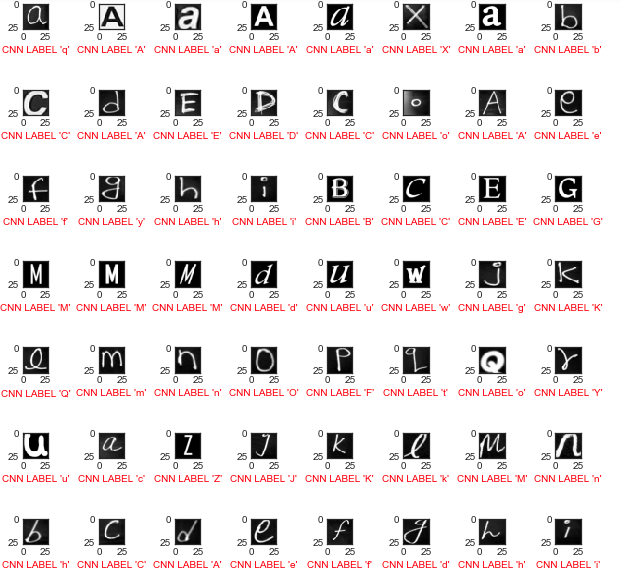
\includegraphics[scale=0.5]{recog}
\caption{Training images for our model}
\end{figure}

Recognition is same as that of testing. The image which is to be recognized is passed into image processor for conversion of it into gray-scaled array of the pixel intensity and passed into predictor function which predicts the label of the image.
\end{itemize}






